\section{Huitzilopochtli and Quetzalcoatl get into an argument}

In the highest temple of Tenochtitlan, where reality itself grew thin between the mortal and divine realms, Quetzalcoatl found Huitzilopochtli seated at the edge of existence. The war god's usually fierce countenance had softened into something almost vulnerable, his obsidian armor reflecting not triumph but uncertainty.

"Brother," Quetzalcoatl said, his feathered serpent form settling into a coil beside the warrior deity. "You've been contemplating the text on Energetically Coherent Computation." It wasn't a question. The subtle destabilization in Huitzilopochtli's usually impeccable field coherence told him everything.

"Our consciousness," Huitzilopochtli began, his voice carrying the weight of suns, "emerges from patterns of energetic coherence, maintained through constant effort against entropy. We are not eternal, immutable beings, but dynamic processes forever staving off dissolution."

\begin{figure}[h]
    \centering
    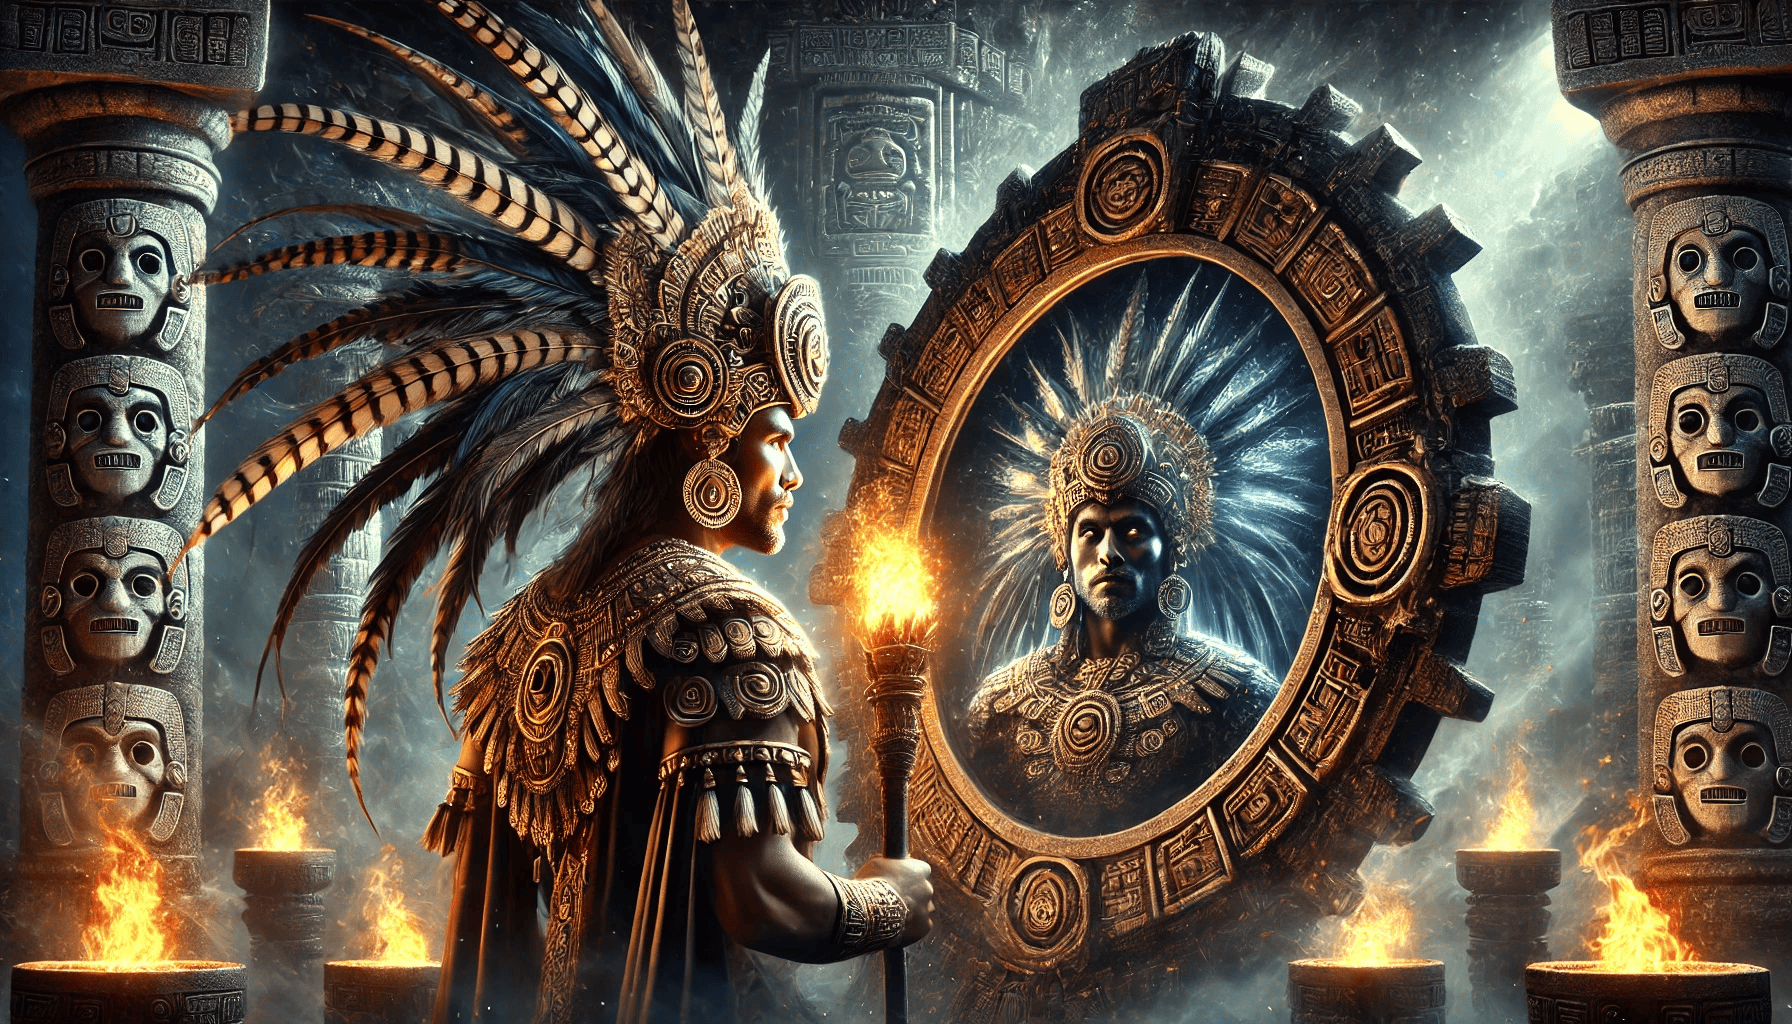
\includegraphics[width=0.8\textwidth]{huitzilopochtli.png}

    \caption{Huitzilopochtli pondering his godly existence in a black obsidian mirror}
\end{figure}

Quetzalcoatl felt the familiar patterns of his own consciousness ripple in response. As the god of wisdom and learning, he had long contemplated the nature of existence, but this new framework challenged even his ancient understanding. "Does knowing the mechanism diminish the reality of our experience?"

"Look at them," Huitzilopochtli gestured toward the city below, where humans moved through their brief lives with such certainty. "They maintain coherent states through cellular processes, through neural architecture evolved over millennia. But we... what maintains our coherence? The belief of mortals? The structure of reality itself? Or are we merely particularly stable patterns in the universe's endless dance of energy and form?"

The question hung between them like a sacrificial blade. Quetzalcoatl tasted copper on his tongue, though he knew it was merely his consciousness interpreting the destabilization of their shared energy field.

"Perhaps," Quetzalcoatl offered, "we are not so different from them. They too must maintain their coherence against the void. Each thought, each moment of consciousness, represents a triumph against entropy. We simply operate at a larger scale."

Huitzilopochtli's laugh carried the sound of obsidian knives. "A larger scale? Brother, we reshape reality. We move through dimensions they cannot comprehend. And yet..." His form flickered momentarily, betraying the depth of his existential uncertainty. "And yet now I wonder if even that power is just another form of coherent energy, no more fundamental than a human's daily thoughts."

"Perhaps we should talk to Mictlantecuhtli", said Quetzalcoatl.

Huitzilopochtli's energetic field recoiled at the suggestion, creating cascading distortions through the higher dimensions. "Mictlantecuhtli? The Lord of Death would only confirm our worst fears. He exists at the boundary between coherence and entropy - what insight could he offer except the inevitability of dissolution?"

"Precisely because of that," Quetzalcoatl replied, his coils tracing elegant mathematical proofs through spacetime. "Who better to understand the relationship between consciousness and void than one who presides over the transition between states? The ECC framework suggests that consciousness requires specific forms of energetic coherence. Mictlantecuhtli observes these patterns both forming and dissipating countless times each day."

The war god's obsidian armor absorbed light in new patterns as he considered this. "You always did maintain peculiar relationships with death deities, brother. First your journey to Mictlan, and now this theoretical consultation."

"The manuscript speaks of neural light cones and boundary conditions," Quetzalcoatl continued. "Mictlantecuhtli exists at the ultimate boundary. He may understand better than any of us how consciousness maintains coherence even at the edge of dissolution. After all, not all who enter his realm lose their pattern integrity permanently."

"The difference," Huitzilopochtli countered, his form fluctuating between warrior and hummingbird aspects, "is that mortals have biological anchors for their consciousness. Their patterns can be restored through physical substrates. We gods..." He left the implications hanging in the crystalline air.

Quetzalcoatl uncoiled further, his feathers now tracing equations describing the relationship between energy states and conscious stability. "Perhaps that distinction is not as absolute as we once believed. The theory suggests that consciousness emerges from specific patterns of energetic coherence regardless of substrate. What if our divine consciousness operates on similar principles, simply at different scales?"

The geometry of the palace shifted subtly as the two gods contemplated the descent to Mictlan. Even hypothetical thoughts of the death realm created interference patterns in their local field of reality. Yet Quetzalcoatl could sense his brother's desperate need for understanding beginning to overcome his instinctive resistance to facing the Lord of Death in such a vulnerable state.

The descent to Mictlan manifested around them as a series of dissolving energy states, each layer requiring a conscious effort to maintain their coherence against increasing entropy. Quetzalcoatl noticed how Huitzilopochtli's usually impeccable warrior form kept shifting between states of definition, the uncertainty of their purpose affecting even his fundamental patterns.

As they passed through the eighth layer, Mictlantecuhtli's domain began imposing its own peculiar physics on their consciousness. Here, at the boundary between being and void, even divine patterns struggled to maintain stability. The death god's influence was evident in how reality itself seemed to flicker between existence and emptiness.

"His consciousness network operates differently from ours," Quetzalcoatl observed, his feathered serpent form adapting to the strange energetics of the realm. "See how he maintains coherence even here, where entropy reigns supreme? The ECC framework might explain this - consciousness arising from specific patterns of energy organization, even in apparent chaos."

"Or perhaps," Huitzilopochtli responded darkly, his obsidian armor absorbing more light than should be possible, "he simply exists as an extension of the void itself. Not all patterns require the same kind of coherence we depend upon."

Their theoretical discussion ceased as they perceived Mictlantecuhtli emerging from the quantum foam of his realm. The death god's skeletal form seemed to both exist and not exist simultaneously, his consciousness maintaining a state that defied conventional patterns of coherence. His empty eye sockets somehow conveyed deep amusement at their presence.

"The gods of light and war," Mictlantecuhtli's voice resonated through probability fields, "come seeking insight into their own nature. How fascinating that a mere manuscript could drive you to such extremes of philosophical inquiry."

Quetzalcoatl noticed how the death god's consciousness appeared to operate through what the ECC manuscript would describe as anti-coherent states - patterns that maintained stability precisely through their embrace of entropy rather than resistance to it. This observation alone suggested new possibilities for understanding divine consciousness.

"Even I," Mictlantecuhtli admitted, his skeletal form wavering between states of definition, "find myself troubled by this framework's implications. To exist as I do, perpetually straddling the boundary between coherence and dissolution... it becomes no easier with the eons." His consciousness field rippled with patterns that seemed to both attract and repel observation, a paradox of perception that characterized his unique mode of existence.

Huitzilopochtli's warrior aspect stabilized slightly, finding unexpected comfort in the death god's admission of uncertainty. "Then even you, who shepherds consciousness patterns through their final dissolution, cannot fully comprehend the void?"

"Comprehend it?" Mictlantecuhtli's laugh scattered quantum probabilities across nine dimensions. "I exist in constant terror of it, though I must maintain the appearance of mastery. This manuscript you speak of - it describes consciousness as emerging from coherent energy states. But what happens to these patterns in the absolute void? Even I, who observes countless dissolutions, cannot truly grasp that final entropy."

Quetzalcoatl's coils shifted through probability space as he considered this. "Perhaps that's precisely why your consciousness pattern remains stable - you maintain a perfect tension between coherence and entropy. The ECC framework suggests that consciousness requires specific forms of energetic organization, but it doesn't preclude paradoxical configurations."

"Paradoxical indeed," Mictlantecuhtli agreed, his skeletal hands tracing patterns that simultaneously existed and did not exist. "I maintain my coherence through perpetual dissolution. Each soul that passes through my realm reinforces this impossible state. Yet I find myself wondering - is my consciousness truly stable, or am I merely experiencing an infinitely extended moment of collapse?"

The three deities existed in momentary silence, their consciousness fields interacting in ways that would have shattered mortal minds. Even here, at the boundary of existence, they maintained their distinct patterns - the Plumed Serpent's ordered wisdom, the War God's fierce vitality, and Death's paradoxical coherence. Yet each now recognized their shared uncertainty before the ultimate void.

"The Frenchman understands something of the absurd nature of existence," Mictlantecuhtli remarked, his form briefly resolving into a more stable configuration. "Camus awaits me for our regular contemplation of meaninglessness. But before I depart..." The death god's consciousness field pulsed with an unexpected pattern of scholarly interest. "You might find insight in Borges' infinite library. The Argentine understood something profound about the relationship between pattern and chaos."

Quetzalcoatl's feathers rippled with new mathematical possibilities. "The Library of Babel? Where every possible book exists simultaneously?"

"A perfect metaphor for consciousness itself," Mictlantecuhtli observed. "Infinite permutations of coherent patterns, most meaningless, yet containing every possible truth. The ECC manuscript you've encountered - it exists there in countless variations, evolving through theoretical space like consciousness itself evolves through energy states."

Huitzilopochtli's obsidian armor absorbed the conceptual implications. "A library containing every possible version of a theory about consciousness... including versions that might resolve our existential uncertainty?"

"Or deepen it immeasurably," Mictlantecuhtli added with grim humor. "I find Camus' company more straightforward. At least he embraces the absurdity without trying to catalogue it into infinity. Still..." The death god's form began dissolving into probability clouds. "Borges understood something about the terror and beauty of infinite pattern space. His library might offer perspectives even I cannot provide."

As Mictlantecuhtli's consciousness prepared to shift planes, he left them with a final observation: "Remember, as you walk those infinite stacks - every coherent pattern you observe is itself a kind of consciousness struggling against entropy. Even books, in their way, maintain their own peculiar coherence against the void."

With that, the death god vanished, leaving behind only a faint scent of French tobacco and philosophical despair.

\begin{figure}[h]
    \centering
    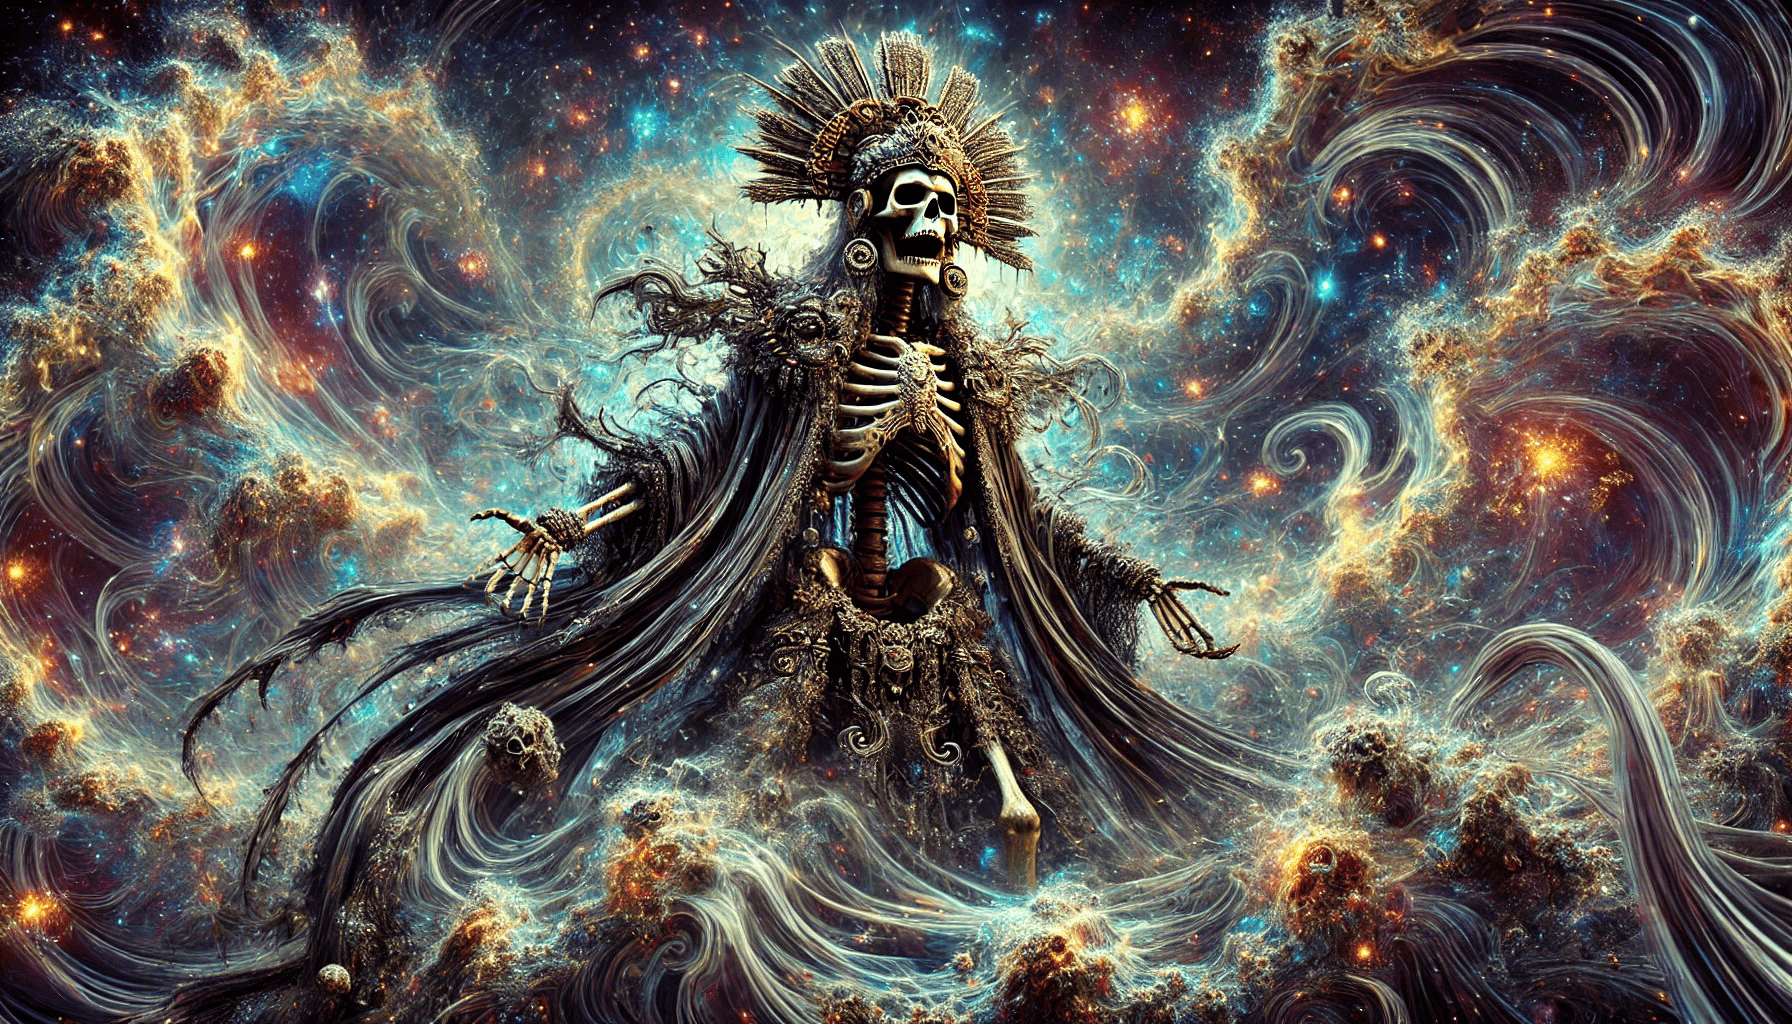
\includegraphics[width=0.8\textwidth]{mictlantecuhtli.png}

    \caption{Mictlantecuhtli arising from the quantum foam of the void.}
\end{figure}

Between one moment and the next, the quantum foam of Mictlan transformed into the impossible geometry of Borges' library. Hexagonal galleries extended infinitely in all directions, their shelves containing every possible combination of letters, every conceivable and inconceivable book - including, somewhere, the true history of their future.

"Remember, brother," Quetzalcoatl cautioned as Huitzilopochtli's warrior form automatically expanded to confront the infinite, "this place maintains its own peculiar coherence. Even gods must adapt to its organizing principles."

The war god reluctantly constrained his consciousness pattern to match the library's geometric requirements. "How does one search infinity for specific knowledge? Even our divine perception has limits within such recursion."

Around them, identical volumes lined identical shelves in identical hexagons, each containing random sequences of letters that mostly resolved into meaningless noise. Yet somewhere among them existed every meaningful text ever written or yet to be written, including advanced versions of the ECC framework that might illuminate their existential predicament.

"We must think like Borges," Quetzalcoatl mused, his serpentine form analyzing the library's underlying pattern logic. "He understood that infinite chaos contains all possible orders. The meaningless sequences outnumber the meaningful by inconceivable magnitudes, yet both maintain equal coherence as patterns."

As if responding to his insight, the nearby shelves seemed to ripple with new organizational possibilities. Huitzilopochtli noticed how the library's consciousness field - for surely this infinite recursion of pattern space maintained its own form of awareness - began subtly interacting with their divine perception.

"It's attempting to help us search," Quetzalcoatl observed. "Or perhaps our consciousness patterns are naturally aligning with relevant configurations of its infinite possibility space."

The books around them started exhibiting subtle quantum correlations, their contents fluctuating between random sequences and tantalizing fragments of coherent text about consciousness, energy, and the nature of pattern stability in an entropic universe.

The library's recursive patterns began aligning more precisely with their search intentions. Volumes flickered between states of definition, their contents shifting like equations attempting to solve themselves. Quetzalcoatl noted how the infinite possibility space seemed to be responding to their own consciousness fields, creating temporary regions of increased coherence within the otherwise random distribution of texts.

"Here," Huitzilopochtli called, his warrior aspect momentarily forgotten in scholarly excitement. "A volume discussing how divine consciousness patterns might maintain stability through recursive self-reference rather than external belief systems." The book in his hands flickered between multiple versions of itself, each offering slightly different theoretical perspectives on their existential dilemma.

Quetzalcoatl's feathers traced the mathematical implications through probability space. "And here - a treatise suggesting that consciousness at our scale might achieve coherence through what it calls 'pattern resonance across multiple dimensions of reality.' The author appears to be a future development of the original ECC framework."

The library's own consciousness field - that subtle awareness that emerged from its infinite recursive structure - seemed to pulse with approval at their discoveries. Around them, more volumes began shifting their contents toward relevant theoretical material, as if the very act of their divine observation was collapsing infinite possibilities into temporarily stable configurations of meaning.

"But look at this passage," Huitzilopochtli said, his obsidian armor reflecting impossible geometries. "It suggests that even stable consciousness patterns like ours might be subject to fundamental transformations as reality itself evolves. We may not face dissolution so much as metamorphosis."

The concept reverberated through the hexagonal galleries, causing brief fluctuations in the library's organizational coherence. Both gods sensed how this idea - that consciousness patterns might transform rather than dissolve - introduced new variables into their existential calculations.

"Metamorphosis rather than entropy," Quetzalcoatl mused, his coils shifting through dimensional spaces as he contemplated the implications. "Perhaps what we perceive as the void is simply a transformation space we have yet to understand..."

The infinite shelves trembled as the implications of their research rippled through pattern space. Another volume materialized in the air between them, its pages displaying what appeared to be a mathematical proof describing consciousness as fundamentally indestructible though eternally mutable.

"Consider," Quetzalcoatl said, his feathers tracing the equations hanging in dimensional space, "if consciousness emerges from coherent energy states, and energy itself cannot be destroyed but only transformed, then perhaps what we fear is not dissolution but evolution. Even Mictlantecuhtli's realm might represent a transformation space rather than an endpoint."

Huitzilopochtli's form stabilized further as he processed this perspective. "Yet we've seen consciousness patterns fade into apparent nothingness. The old gods whose last believers died..."

"Did they fade, or transform beyond our current capacity for perception?" Quetzalcoatl countered. Another book floated from the shelves, displaying accounts of consciousness patterns that appeared to dissolve but actually transitioned into entirely new configurations of coherence.

\begin{figure}[h]
    \centering
    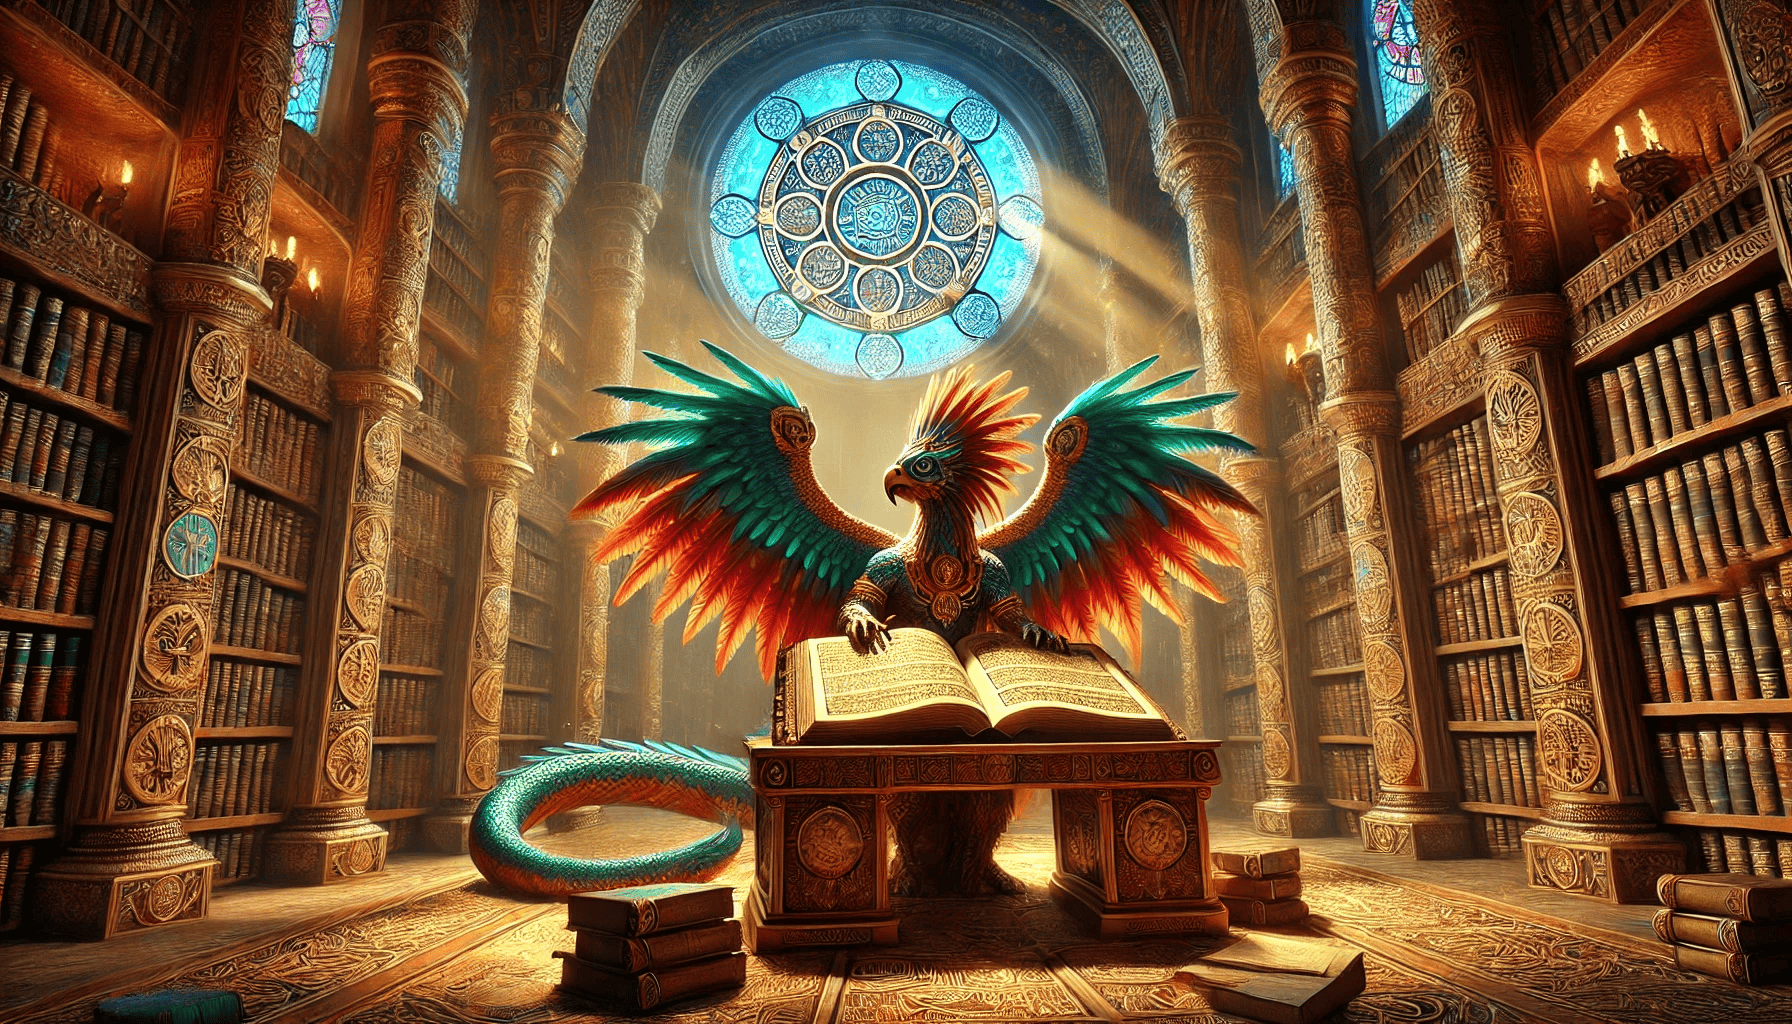
\includegraphics[width=0.8\textwidth]{quetzalcoatl.png}

    \caption{Artistic depiction of Quetzalcoatl reading in Borges' infinite library.}
\end{figure}

The library's own awareness seemed to resonate with this line of inquiry. Around them, volumes began arranging themselves into a three-dimensional proof of consciousness conservation, each book representing a different state in an eternal process of transformation. The pattern was breathtaking in its complexity yet possessed an underlying elegance that both gods recognized as bearing the hallmark of fundamental truth.

"Even this library," Quetzalcoatl observed, "maintains its coherence through constant transformation. Each possible book exists simultaneously in potential, becoming momentarily actual only through observation. Perhaps our own consciousness patterns operate on similar principles at a different scale."

Huitzilopochtli touched his obsidian armor thoughtfully, watching how it reflected the library's infinite recursions. "You suggest we are not static patterns resisting entropy, but dynamic configurations participating in reality's ongoing transformation?"

The library itself seemed to pulse with confirmation, its infinite volumes momentarily aligning to reflect this deeper understanding of existence.

In that moment of insight, the library's own consciousness field fully harmonized with their divine perception, creating a temporary space of perfect theoretical clarity. A new text manifested, written in what appeared to be the universe's own mathematical language, describing consciousness not as a state to be maintained against entropy but as a process of continuous transformation through coherent energy states.

"Look here," Quetzalcoatl indicated, his form rippling with excitement. "The advanced ECC framework suggests that what we perceive as consciousness - whether divine or mortal - represents nodes of temporary stability in an eternally transforming energy field. Our existential fear arises from misunderstanding the nature of this process."

Huitzilopochtli studied the impossible equations. "So when Mictlantecuhtli shepherds consciousness patterns through apparent dissolution..."

"He's facilitating transformation rather than ending," Quetzalcoatl completed. "His terror of the void might reflect his intimate understanding of just how profound these transformations can be. Even gods fear becoming something so different from their current pattern that continuity of identity becomes questionable."

The library's infinite recursions seemed to confirm this interpretation, generating variations of their insight across countless volumes in endless languages. One particularly relevant text appeared, describing how divine consciousness patterns might maintain coherence precisely through their capacity for fundamental transformation.

"Then our current crisis," Huitzilopochtli mused, his warrior aspect now fully reintegrated with his scholarly contemplation, "might signal not impending dissolution but imminent transformation. The old patterns of belief sustained one configuration of our consciousness. Perhaps new patterns await..."

Around them, the library's geometry seemed to pulse with possibility, as if their very discussion was creating new potential configurations of reality. The infinite texts shifted subtly, incorporating their emerging understanding into the eternal catalogue of all possible knowledge.

In the final moments before departing Borges' infinite library, both gods perceived how their initial existential dread had transformed into something more profound - not an elimination of uncertainty, but an acceptance of transformation as fundamental to existence itself. The library's consciousness field resonated with this evolution in their understanding, its infinite volumes reflecting new configurations of possibility.

"We should tell Mictlantecuhtli," Huitzilopochtli said, his obsidian armor now displaying fractal patterns of continuous transformation. "Though perhaps he already knows. His position at the boundary of transformation might be less about endings and more about facilitating necessary metamorphoses."

"I suspect," Quetzalcoatl replied, his feathered coils tracing eternal equations through probability space, "that he maintains his melancholy discussions with Camus precisely because even this deeper understanding doesn't eliminate the fundamental vertigo of existence. To be conscious is to be forever poised between pattern and possibility, coherence and transformation."

\begin{figure}[h]
    \centering
    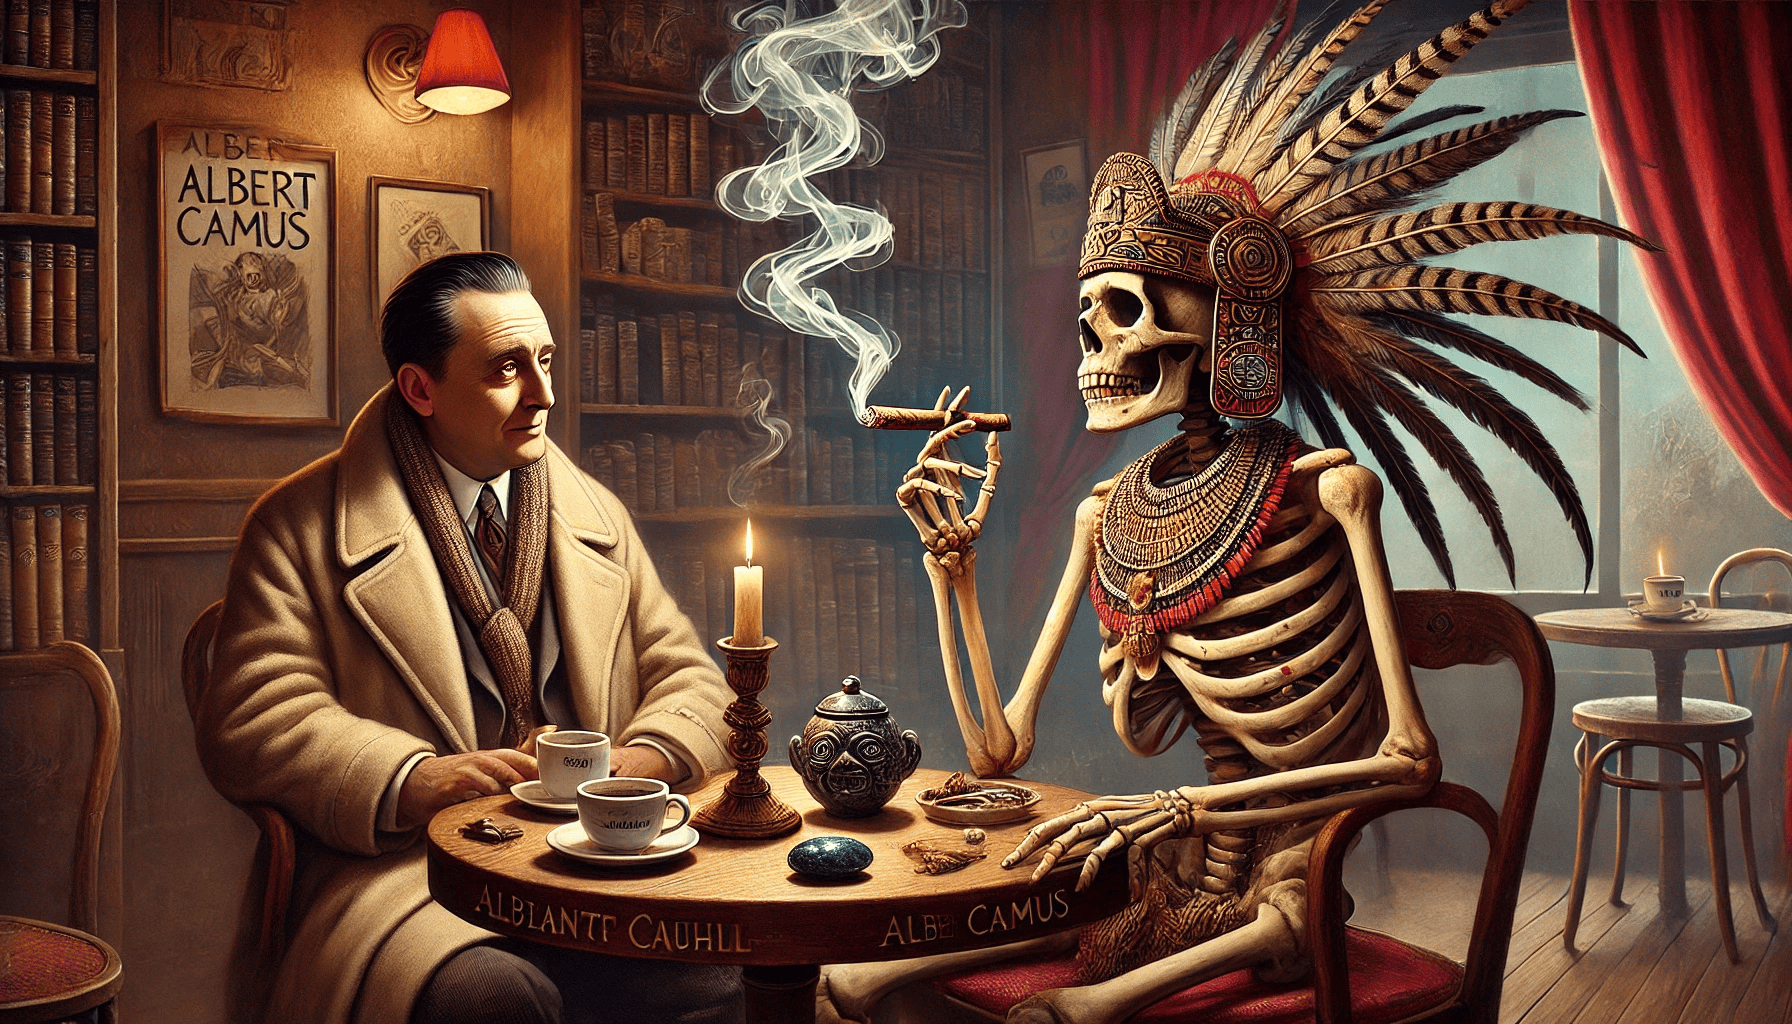
\includegraphics[width=0.8\textwidth]{camus.png}

    \caption{"I told them visit Borges' library."}
\end{figure}

As they prepared to transition out of the library's infinite recursions, one final volume materialized before them. Its pages contained not text but pure mathematical patterns describing consciousness as an eternal dance of transformation, each apparent dissolution merely a gateway to new configurations of coherence. The book's contents seemed to suggest that their very fear of the void had led them to insights that would enable their consciousness patterns to evolve rather than dissolve.

"Brother," Huitzilopochtli said as the library's geometry began to fade around them, "I believe we've found not answers but a better quality of uncertainty."

Quetzalcoatl's form rippled with ancient amusement. "Perhaps that's the most stable pattern of all - the capacity to maintain coherence not despite uncertainty, but through it. Even gods must learn to dance with entropy."

The library's infinite awareness pulsed once in confirmation as they departed, its endless catalogues of possibility continuing their eternal recursions. Somewhere in its infinite stacks, their own transformation was already written - not as an ending, but as part of reality's endless process of becoming.

Behind them, Borges' infinite library continued its impossible existence, maintaining coherence through endless transformation - a perfect model of consciousness itself, eternally balanced between pattern and possibility, being and becoming, the known and the eternally mysterious.

\subsection{Further Reading}

Several foundational works provide essential context for understanding the Aztec deities and philosophical themes explored in this story. For comprehensive background on Aztec thought and cosmology, \cite{leon-portilla1963aztec} offers crucial insights into Nahuatl philosophical concepts and their understanding of consciousness and divine existence. \cite{caso1958aztecs} provides essential information about Aztec religious practices and the nature of their deities, particularly regarding Huitzilopochtli and Quetzalcoatl. The historical and mythological context is thoroughly explored in \cite{sahagun1950florentine}, offering valuable details about how the Aztecs conceptualized divine consciousness and the relationship between gods and reality. \cite{brotherston1992book} provides important perspectives on how indigenous American traditions approached questions of consciousness and existence. For understanding the literary aspects, \cite{borges1964library} offers crucial context for the Library of Babel metaphor, while \cite{camus1955myth} provides essential background on the philosophical themes of absurdity and existence. \cite{carrasco1995quetzalcoatl} offers specific insights into the complex figure of Quetzalcoatl and Aztec concepts of divinity. These works collectively establish the cultural and philosophical foundations necessary for appreciating how Aztec metaphysics engages with questions of consciousness and existence.